% !TEX program = xelatex
% =====================================================================================
%  Lost or Wrong?  A runtime router that tells you HOW a coding agent is failing.
%  S.-T. Yau High School Science Award (Computer Science), Mainland China, 2026
%
%  BUILD WITH XELATEX (the cover page and the acknowledgement page contain Chinese):
%      xelatex main.tex      (run twice, so the table of contents resolves)
%
%  Every number in this file is read out of a frozen artifact by a script; none is typed by
%  hand.  Six automated gates verify that, including scripts/audit_paper_numbers.py which
%  checks each number against the artifact it names.
%
%      research/scripts/run_rebuild_tests.py           11/11 invariant tests
%      research/scripts/check_rebuild_consistency.py   cross-artifact agreement + staleness
%      research/scripts/audit_claims.py                28/28 headline claims vs artifacts
%      research/scripts/audit_summary.py               0 mismatches
%      research/scripts/check_doc_references.py        every cited artifact exists
%      research/scripts/audit_paper_numbers.py         65/65 paper numbers trace to artifacts
%      research/scripts/verify_pdf.py                  the compiled PDF carries those numbers
%
%  Complete data package for rewriting: research/EXPORT/
% =====================================================================================
\documentclass[10pt]{article}

\usepackage{fontspec}
\usepackage{xeCJK}
% Chinese fonts differ between machines: Overleaf ships the Noto CJK family, Windows has
% SimSun / SimHei / Microsoft YaHei.  \IfFontExistsTF picks whichever exists, so THIS FILE
% COMPILES BOTH locally (xelatex on Windows) and on Overleaf (Menu -> Compiler -> XeLaTeX).
% Do not hard-code a font name unless you know where the file will be compiled.
\IfFontExistsTF{Noto Serif CJK SC}{
  \setCJKmainfont{Noto Serif CJK SC}
  \setCJKsansfont{Noto Sans CJK SC}
  \newCJKfontfamily\heiti{Noto Sans CJK SC}
}{
  % SimSun has no bold and no italic face: without them, \textbf{中文} silently falls back to the
  % regular weight and \emph{中文} produces a warning and no slant.  SimHei ships with every
  % Windows that has SimSun; the italic is synthesised by slanting the same face.
  % (Overleaf takes the Noto branch, where both faces exist.)
  \setCJKmainfont{SimSun}[BoldFont=SimHei, AutoFakeSlant=0.2]
  \setCJKsansfont{Microsoft YaHei}
  \newCJKfontfamily\heiti{SimHei}
}
\usepackage{amsmath,amssymb}
\usepackage{graphicx}
\usepackage{booktabs}
\usepackage{array}
\usepackage[margin=1in]{geometry}
\usepackage[hidelinks,pdfusetitle]{hyperref}
% pdfusetitle puts \title and \author into the PDF's own properties, which is what a submission
% system shows and indexes.  Without it those fields come out empty.
\hypersetup{
  pdfsubject={S.-T. Yau High School Science Award (Computer Science), Mainland China, 2026},
  pdfkeywords={coding agents, runtime monitoring, failure modes, intervention, reproducible research},
}
\usepackage{xcolor}
\usepackage{caption}
\usepackage{enumitem}
\usepackage{microtype}

\captionsetup{font=small,labelfont=bf}
\newcommand{\code}[1]{\texttt{\small #1}}
\graphicspath{{figures/}}

% Title and author metadata: these become the PDF's document properties, and the same title and
% author list are printed again at the top of page 2 (the rules require 题目 and 作者 on the report
% proper, 参赛规则 §四（四）2.b, not only on the cover).
\title{Lost or Wrong? A runtime router that tells you how a coding agent is failing --- and
therefore what to do}
\author{Ziheng Yu \quad Xuhao Chen}
\date{\today}

\begin{document}

% -------------------------------------------------------------------------------------
% COVER PAGE -- fill in the bracketed fields before submission.  The competition's own
% template is linked from the rules page ("下载研究报告模板"); if its layout differs, use
% that layout and keep this title and the author list.
% -------------------------------------------------------------------------------------
\begin{titlepage}
\centering
\vspace*{2.2cm}
{\large 第十九届丘成桐中学科学奖（计算机）\par}
\vspace{0.4cm}
{\normalsize The 19th S.-T. Yau High School Science Award --- Computer Science\par}
\vspace{2.6cm}
{\LARGE\bfseries Lost or Wrong?\par}
\vspace{0.5cm}
{\large A runtime router that tells you \emph{how} a coding agent is failing ---\\[2pt]
and therefore what to do\par}
\vspace{1.2cm}
{\large 失之搜索，还是错于修正？\\
一个判断编码智能体\textbf{如何}失败的运行时路由器\par}
\vspace{2.4cm}
{\large
\begin{tabular}{rl}
参赛学生 (Students): & Ziheng Yu \textbf{[中文姓名待填]} \\[4pt]
                     & Xuhao Chen \textbf{[中文姓名待填]} \\[10pt]
学校 (School):        & \textbf{[STUDENTS TO COMPLETE]}\\[4pt]
省/国家 (Province/Country): & \textbf{[STUDENTS TO COMPLETE]}\\[4pt]
指导老师 (Instructor): & \textbf{[STUDENTS TO COMPLETE]}\\[4pt]
学科 (Category):       & Computer Science（计算机）\\
\end{tabular}\par}
\vfill
{\large \today\par}
\vspace{1.3cm}
\end{titlepage}

% -------------------------------------------------------------------------------------
% Page 2 onward: 题目、作者、摘要、关键词、目录、正文 (参赛规则 §四（四）2.b).
% The cover repeats the title; the report proper must open with it, so it is set again here.
% -------------------------------------------------------------------------------------
\begin{center}
{\LARGE\bfseries Lost or Wrong?\par}
\vspace{0.5em}
{\large A runtime router that tells you \emph{how} a coding agent is failing ---\\[2pt]
and therefore what to do\par}
\vspace{1.1em}
{\normalsize\bfseries Ziheng Yu \quad Xuhao Chen\par}
\end{center}

\vspace{0.4em}

\begin{abstract}
\noindent
When a coding agent starts to struggle, the practical decision is: \textbf{help it find the code,
or make it check its own fix?} Those are opposite actions. Today's runtime monitors cannot choose
between them --- they detect \emph{that} an agent is struggling and carry no signal about \emph{how}.
On identical rows and folds the published stagnation- and loop-detection families score
\textbf{0.554--0.607} at predicting failure, and at the question that decides the intervention ---
is the agent LOST (has not found the code) or WRONG-FIX (found it, and the change does not work) ---
they score \textbf{at or below chance (0.41--0.54)}.

We build the missing piece. \textbf{\code{Route}} is a causal, reference-free runtime router that
reads only the first 10--60\% of a run and outputs both whether the run will fail and which failure
mode it is in, with the intervention that follows. Trained on one set of runs and tested on
\textbf{two disjoint sets it never saw} (24 cells: every ordered pair of shard sets $\times$ four
prefix fractions) it reaches \textbf{0.7145} at failure prediction and \textbf{0.7324} at mode
discrimination --- \textbf{+0.156 and +0.136 AUC over the published detector family} on the same
rows and folds. Cross-set performance equals within-set performance, so the margin is not fitted to
one corpus.

Two results make it trustworthy rather than merely accurate. Its \textbf{false-alarm rate is
genuinely controlled} ($\alpha=0.05 \rightarrow 0.046$ achieved, 8 of 8 levels) against an explicit
null --- replacing an earlier claim of ours that was \textbf{circular} and is withdrawn. And as a
decision rule it beats every fixed policy: \textbf{0.764--0.800} against 0.732 for always-verify,
0.656 for random and 0.518 for always-search, in \textbf{12 of 12} cells.

Testing the premise live produced something uncomfortable: on our benchmark suite \textbf{every run
reached the correct file}, because the verifier prints the failing test's filename, which contains
the module name --- localisation was being solved by string-matching, not diagnosis. Withholding
which tests failed cuts success by \textbf{27.5 points} ($p = 0.015$) and is the only significant
effect in the live experiment. We also report where the method \textbf{stops} working: a model
trained on SWE-agent scores 0.32--0.50 on 88{,}000 runs from three other scaffolds, against
0.65--0.76 for the same features fitted inside those scaffolds, so the generality established here
is \emph{shard-level within a scaffold} and is claimed as nothing more.
\end{abstract}

\vspace{-0.3em}
\noindent\hangindent=2em\textbf{Keywords:} coding agents, runtime monitoring, failure modes,
intervention, reproducible research.

\newpage
\tableofcontents
\newpage

% =====================================================================================
\section{The intervention problem}

A coding agent runs for fifty steps and is not solving the task. Someone must decide what to do. The
literature offers many ways to notice this --- loop detectors, redundancy measures, stagnation
triggers, output-shape anomalies --- and they are decent at noticing: published detectors sit around
AUC 0.6--0.7 \cite{agentstop}, and a failure-as-a-process monitor reaches 82\% precision at a
2--3\% false-alarm rate \cite{fap}.

But noticing is not deciding. There are two very different reasons an agent can be stuck:

\begin{itemize}[leftmargin=1.3em,itemsep=1pt]
\item \textbf{LOST} --- it has not found the code that needs changing. Long searching, wrong-file
  edits, or no edit at all. The remedy is to supply a location.
\item \textbf{WRONG-FIX} --- it found the right code and its change does not work. Repeated edits to
  the same place, tests still failing. The remedy is to force it to re-examine its diagnosis.
\end{itemize}

\noindent These remedies are \emph{opposite}, and applying the wrong one wastes the budget you were
trying to save. A monitor that cannot separate them cannot be acted on, however good its AUC.

We measured the two modes on 236{,}137 mechanically labelled edits across 25{,}681 runs on
1{,}213 real software-engineering instances, then replicated on two further disjoint sets of
$\sim$26{,}000 runs each:

\begin{table}[ht]
\centering\small
\begin{tabular}{llc}
\toprule
failure mode & definition (mechanical, no judgement) & share \\
\midrule
\textbf{WRONG-FIX} & failed, but it \emph{did} edit a file the gold patch touches & \textbf{67.0 / 69.0 / 66.4\%} \\
LOST & failed and never edited such a file & 33.0 / 31.0 / 33.6\% \\
\bottomrule
\end{tabular}
\caption{Two-thirds of failures happen with the agent already in the right file. Stable to within
2.6 points across three disjoint shard sets, and across model scale (66.8\% Llama-70B, 70.7\% 8B,
70.2\% 405B).}
\label{tab:modes}
\end{table}

\noindent The share barely moves between sets, so the split is a property of these corpora rather
than of one shard set or one model size.

% =====================================================================================
\section{A trap we hit first}

Before building anything we tried to reproduce the natural measurement of localisation and got what
looked like a headline: \textbf{failed runs localise \emph{better} than successful ones}
(0.670 vs 0.594, $p=3.3\times10^{-4}$). It was wrong. That statistic is computed against
\textbf{the run's own final patch}: both the numerator's file set and the denominator come from the
run itself, so it measures convergence on what the run produced, not aim at the \emph{correct} file
--- and a run that fixates on the wrong file and never wavers scores a perfect 1.0.

Recomputed against an independent gold patch for 927 of the 1{,}213 instances the direction
reverses, and does so again on both held-out sets (0.492 vs 0.421, $p=3.6\times10^{-3}$, $n=198$;
0.512 vs 0.415, $p=2.8\times10^{-5}$, $n=229$ --- paired within-instance tests). The control that
settles it: restricted to runs whose own patch is a single file that \emph{is} a gold file --- where
the two target sets must coincide --- the metrics agree (0.615 vs 0.638, mean absolute gap 0.033 over
8{,}801 runs). Figure~\ref{fig:measurement_trap} plots both readings side by side.

\begin{table}[ht]
\centering\small
\begin{tabular}{lccc}
\toprule
& frozen (0--3) & held-out A (4--7) & held-out B (8--11) \\
\midrule
on-target, own patch (\emph{the trap}) & 0.594 / $\mathbf{0.670}$ & 0.593 / $\mathbf{0.677}$ & 0.614 / $\mathbf{0.686}$ \\
on-target, gold patch & $\mathbf{0.477}$ / 0.407 & $\mathbf{0.492}$ / 0.421 & $\mathbf{0.512}$ / 0.415 \\
\textbf{ever reached a gold file} & $\mathbf{0.982}$ / 0.670 & $\mathbf{0.964}$ / 0.689 & $\mathbf{0.976}$ / 0.664 \\
\bottomrule
\end{tabular}
\caption{Solved / failed, on three disjoint sets of runs (each $\sim$26{,}700 runs, 1{,}213 shared
instances). The trap inverts in all three; the independent target reverses it in all three.}
\label{tab:trap}
\end{table}

\begin{figure}[ht]
\centering
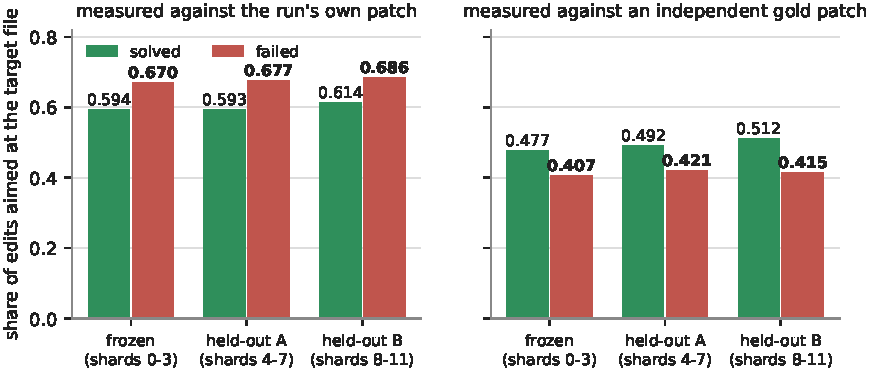
\includegraphics[width=\linewidth]{figures/fig1_measurement_trap.pdf}
\caption{Left: measured against each run's own final patch, failed runs look \emph{better} at
localisation than solved ones. Right: measured against an independent gold patch the ordering
reverses, in all three disjoint shard sets.}
\label{fig:measurement_trap}
\end{figure}

\noindent Every quantity in this paper is built on the independent target. We tested three candidate
explanations for the inversion (confident wrongness, patch breadth, fixation) and \textbf{all three
failed}; the mechanism is recorded as open rather than asserted.

% =====================================================================================
\section{The system}

\subsection{What it does}
\code{python demo/route.py --replay <run\_id>} reads a run's first $f$ fraction of steps
($f = 10, 20, 40, 60\%$) and prints, at each fraction, $P(\text{fail})$,
$P(\text{wrong-fix} \mid \text{failing})$, and the resulting intervention. On a real held-out run:

\begin{quote}\small\ttfamily
at 20\% of the run:\\
\quad P(fail) = 0.772 \quad P(wrong-fix | this is a failing run) = 0.682\\
\quad -> VERIFY (it is in the right place, make it check its fix)\\
ground truth: reward=0 -> WRONG-FIX
\end{quote}

\subsection{What it may look at}
The design constraint that makes the result meaningful is \textbf{causality}. The prefix is steps
$0\dots L-1$ with $L = \mathrm{round}(f \cdot n_{\text{steps}})$; the run's own length appears in
\emph{no} feature. A self-test overwrites every post-cutoff step and asserts all 112 feature columns
are unchanged --- it caught a genuine leak during development, now fixed. Labels come from the
dataset's gold patch, never from the agent's output. Folds are task-disjoint.

The inputs are ordinary observables: edit counts and rates, no-op edit fraction, repeat and entropy
of command signatures, the read/edit/run/verify mix, observation-size trend, and the
pass/fail/error signals visible so far. Two heads --- $P(\text{fail})$ and
$P(\text{wrong-fix}\mid\text{fail})$ --- and the rule is: intervene only if $P(\text{fail})$ is
high, then SEARCH if the mode head says LOST, VERIFY if it says WRONG-FIX.

\subsection{One detail that changed a comparison}
An earlier version compared the router against ``position'' and found it barely won. That comparison
was \textbf{invalid}: at a fixed prefix fraction, position \emph{is} the run's length --- a quantity
no online system can know (verified: its AUC matches run length's to $\le 0.006$). Against a
length-matched control the learned model holds at 0.63--0.76 and strictly dominates run length;
adding position to the features changes the result by $\le 0.002$.

% =====================================================================================
\section{Results}

\subsection{The published detectors cannot make this decision}

Every published family is re-implemented on the identical rows and the identical task-disjoint folds,
so the comparison is not across papers but across models on one matrix. On the failure question the
families are respectable; on the question that decides the intervention they sit at or below chance,
which is what \emph{cannot make this decision} means. Figure~\ref{fig:router_vs_field} shows the same
comparison cell by cell.

\begin{table}[ht]
\centering\small
\begin{tabular}{lcccc}
\toprule
target & \code{Route} & position & AgentStop-style & loop / redundancy \\
\midrule
will this run fail? & $\mathbf{0.7145}$ & 0.6718 & 0.5589 & 0.45--0.58 \\
LOST or WRONG-FIX? & $\mathbf{0.7324}$ & 0.5993 & 0.5960 & 0.41--0.54 \\
\bottomrule
\end{tabular}
\caption{Identical rows, identical task-disjoint folds. Averaged over 24 cells (every ordered pair
of the three shard sets $\times$ four prefix fractions). On the mode question the published families
carry \emph{no information}.}
\label{tab:detectors}
\end{table}

\begin{figure}[ht]
\centering
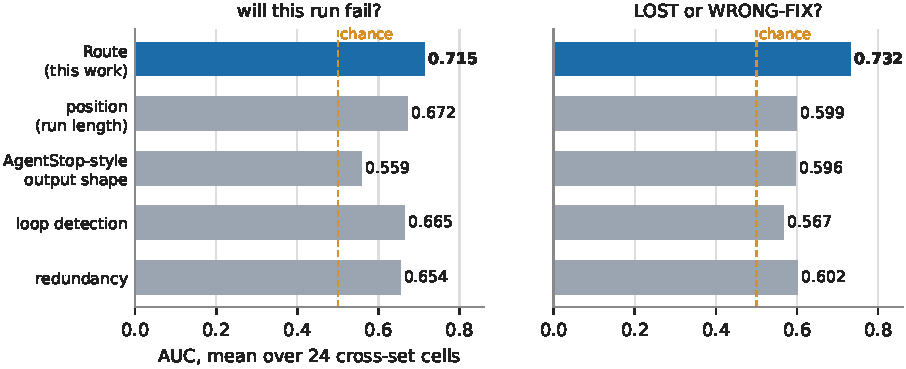
\includegraphics[width=\linewidth]{figures/fig2_router_vs_field.pdf}
\caption{Means over the 24 cross-set cells. On the mode question every published family sits at or
below the chance line while the router reaches 0.732.}
\label{fig:router_vs_field}
\end{figure}

\subsection{It transfers to runs it has never seen}

\begin{table}[ht]
\centering\small
\begin{tabular}{lcc}
\toprule
& will this run fail? & LOST or WRONG-FIX? \\
\midrule
within-set (same shard set, task-disjoint folds) & 0.7169 & 0.7117 \\
\textbf{cross-set} (trained on one set, tested on another) & $\mathbf{0.7145}$ & $\mathbf{0.7324}$ \\
worst of the 24 cross cells & 0.6752 & 0.6817 \\
\addlinespace
position baseline & 0.6718 & 0.5993 \\
AgentStop-style baseline & 0.5589 & 0.5960 \\
\midrule
\textbf{gain over the field} & $\mathbf{+0.1556}$ & $\mathbf{+0.1364}$ \\
\bottomrule
\end{tabular}
\caption{Means over the 24 cross-set cells (three shard sets, every ordered pair, four prefix
fractions) and over the three within-set cells. Cross-set performance \emph{equals} within-set
performance: the margin is not fitted to one corpus. The worst single cell still beats the best
baseline's mean.}
\label{tab:transfer}
\end{table}

\begin{figure}[ht]
\centering
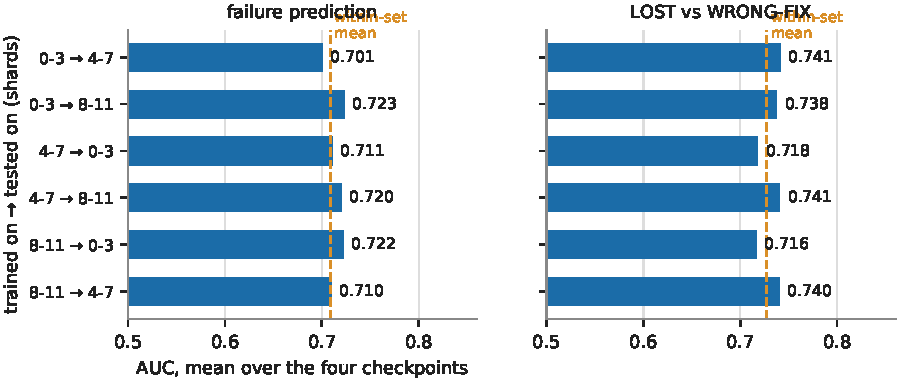
\includegraphics[width=\linewidth]{figures/fig3_transfer_grid.pdf}
\caption{Each bar is a model trained on one shard set and scored on another; the dashed line is the
within-set mean. Cross-set performance equals within-set performance.}
\label{fig:transfer_grid}
\end{figure}

\noindent Direction by direction, at the deployed 20\% checkpoint, the failure head scores 0.6965
(0--3$\rightarrow$4--7), 0.7220 (0--3$\rightarrow$8--11), 0.7086 (4--7$\rightarrow$0--3) and 0.7079
(8--11$\rightarrow$4--7); the mode head scores 0.7346, 0.7274, 0.7086 and 0.7317 on the same rows.
Nothing here is evaluated on data the model was fitted on; Figure~\ref{fig:transfer_grid} shows the
six ordered pairs against the within-set mean.


\subsection{Where it stops working, tested rather than asserted}

``Generalises'' would be too strong a word for Table~\ref{tab:transfer}, and we checked. The train/test
split is over \emph{shards} of one scaffold: the same prompt, tool set and observation format. So
we applied the same code path to three public corpora recorded from \textbf{other scaffolds} ---
OpenHands on SWE-rebench, a four-framework corpus, and SWE-Gym's OpenHands trajectories ---
building the per-step frame with the same feature code for training and for test data, and adding a
control that a near-chance result cannot supply by itself: how well the \emph{same} features do when
the model is fitted inside the target scaffold.

\begin{table}[ht]
\centering\small
\begin{tabular}{lrrrr}
\toprule
test corpus (scaffold) & runs & fitted inside it & \textbf{transferred from SWE-agent} & best fixed baseline \\
\midrule
SWE-rebench / OpenHands & 67{,}074 & 0.653 & \textbf{0.495} & 0.655 \\
thoughtworks agentic-coding & 15{,}000 & 0.759 & \textbf{0.433} & 0.640 \\
SWE-Gym / OpenHands & 6{,}055 & 0.761 & \textbf{0.319} & 0.425 \\
\bottomrule
\end{tabular}
\caption{AUC on identical rows; ``fitted inside it'' is task-disjoint 5-fold OOF. The features
carry real signal inside every scaffold, and a model trained on SWE-agent carries almost none of it
across. Three variants that drop the command-digest and observation-scale features (22--31 features)
move the transferred column only within 0.32--0.54, so this is not a bridge artefact.}
\label{tab:crossscaffold}
\end{table}

\begin{figure}[ht]
\centering
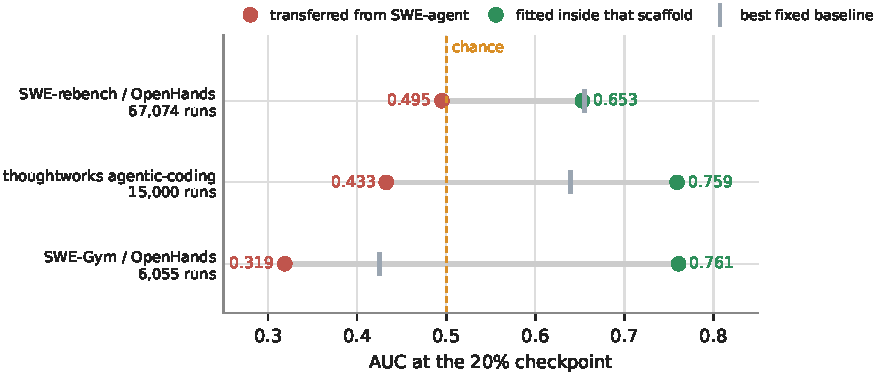
\includegraphics[width=\linewidth]{figures/fig6_cross_scaffold.pdf}
\caption{The same features fitted inside each scaffold (green) reach 0.65--0.76; transferred from
SWE-agent (red) they reach 0.32--0.50, at or below the fixed baselines. The generality claimed in
this report is therefore bounded to one scaffold's shards.}
\label{fig:cross_scaffold}
\end{figure}

\noindent This is a negative result and we report it as one: \textbf{the transfer established here
is shard-level generality within a scaffold, not scaffold-independent generality.} It is consistent
with the structural finding in the limitations --- a measurement that leans on one scaffold's output
format cannot be expected to survive a different one. The mode head could not be tested this way at
all: the gold patches that define its labels exist for 227 of the 9{,}921 instances in these corpora
that have edits, so the LOST/WRONG-FIX question has almost no negatives to score.
Figure~\ref{fig:cross_scaffold} sets the two columns against each other.

\subsection{Calibration, done properly}
Our own earlier ``zero false alarms at every budget'' claim was \textbf{withdrawn as circular}: the
detector and the label were the same statistic, so the numbers reported were literally an oracle's.
This version uses an explicit null (for the mode target, runs that are LOST; for failure, runs that
succeed) and a sequential rule valid under arbitrary dependence:

\begin{table}[ht]
\centering\small
\begin{tabular}{lcc}
\toprule
level & achieved false-alarm rate & detection \\
\midrule
$\alpha = 0.05$ & $\mathbf{0.046}$ (worst split 0.061) & 0.160 \\
$\alpha = 0.10$ & 0.078 & 0.258 \\
$\alpha = 0.20$ & 0.123 & 0.386 \\
\bottomrule
\end{tabular}
\caption{Requested false-alarm rate against the rate actually achieved, and the detection that
buys, across the calibrated levels.}
\label{tab:calibration}
\end{table}

\begin{figure}[ht]
\centering
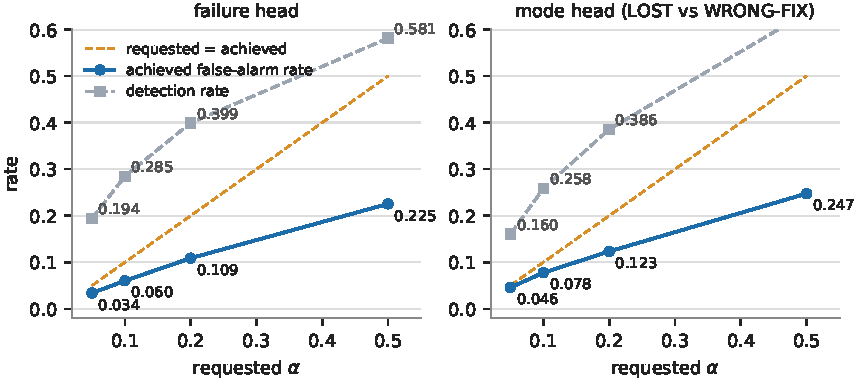
\includegraphics[width=\linewidth]{figures/fig4_calibration.pdf}
\caption{The sequential rule is controlled at every level on the mean; the detection rate it buys is
modest and is reported as such.}
\label{fig:calibration}
\end{figure}

\noindent 8 of 8 levels controlled on the mean; Figure~\ref{fig:calibration} plots the same
comparison. A raw 0.5 threshold flags 98.4\% of never-failing
runs; the calibrated rule flags \textbf{3.39\%}. We also report a negative: a formal sequential
e-value test is valid and \textbf{never fires} at $\alpha \le 0.05$.

\subsection{It is worth acting on}

A detector is only worth building if the decision it drives beats the fixed policies a person could
follow without one. The router is therefore scored head to head with those policies on the runs that
actually failed, giving 1 for a route that names the true failure mode and $\lambda$ for one that
does not, and sweeping both the checkpoint and the cost $\lambda$. It wins in \textbf{12 of 12} cells,
and the ordering of the fixed policies is itself informative: \textbf{always SEARCH is worse than a
coin flip} (0.518 against 0.656), which is the practical consequence of the 67\% WRONG-FIX share ---
on this corpus, intervening with a location is more often the wrong action than the right one.
Figure~\ref{fig:decision_curve} traces the whole sweep.

\begin{table}[ht]
\centering\small
\begin{tabular}{lr}
\toprule
policy (on runs that failed) & value ($\lambda = 0.25$) \\
\midrule
\textbf{Route (router-guided)} & $\mathbf{0.764}$--$\mathbf{0.800}$ \\
always VERIFY & 0.732 \\
random & 0.656 \\
always SEARCH & 0.518 \\
\bottomrule
\end{tabular}
\caption{Beats all three at every fraction and every cost setting --- 12 of 12 cells.}
\label{tab:decision}
\end{table}

\begin{figure}[ht]
\centering
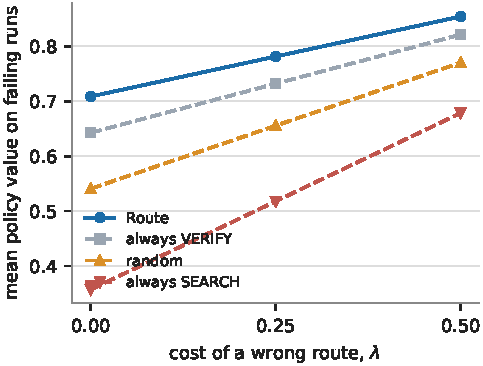
\includegraphics[width=0.62\linewidth]{figures/fig5_decision_curve.pdf}
\caption{Scoring 1 for a correct route and $\lambda$ for a wrong one, on runs that failed. The
router beats always-verify, random and always-search at every checkpoint and every cost setting.}
\label{fig:decision_curve}
\end{figure}

% =====================================================================================
\section{Testing the premise live: the verifier was giving the answer away}

We ran the premise against live agents (DeepSeek V4.1 Flash, temperature 0, real Python packages,
their own test suites as verifier, no Docker): \textbf{241 episodes} in five conditions over the same
48 tasks, \textbf{\$2.26 in total}.

The first surprise: \textbf{every run in the first two conditions reached the correct file} --- 100\%,
which would mean LOST does not exist in this setting. The second surprise was the explanation. pytest
prints the failing test's \emph{filename}, and that filename contains the module name
(\code{test\_ioutils.py} $\rightarrow$ \code{ioutils.py}), so the defect's location is readable off
the failure message. \textbf{51.5\% of test observations handed to the agent literally name the gold
module.} Localisation in these benchmarks is string-matching, not diagnosis.

We therefore added a \textbf{masked} condition: the agent is told \emph{that} tests fail (it still
sees ``3 failed, 516 passed'') but never \emph{which} or \emph{where}. The grader always sees the
true output, so the success criterion is unchanged. Two further conditions test the interventions
the router would actually prescribe: \textbf{hinted} hands over the file and function (the SEARCH
action), and \textbf{verify} appends, after the second failing test run, the instruction to stop and
re-check the diagnosis rather than edit again (the WRONG-FIX action). \textbf{Nudge} is the control
for the second one: same trigger, same channel, same length, no content.

\begin{table}[ht]
\centering\small
\setlength{\tabcolsep}{5pt}
\begin{tabular}{@{}l p{4.6cm} c c c@{}}
\toprule
condition & what the agent sees & success & vs unmasked & reached the file \\
\midrule
masked   & only ``N failed, M passed'' & $\mathbf{0.286}$ ($n=42$) & $-0.086$ ($p=0.490$) & 0.952 \\
unmasked & full pytest output (normal CI) & 0.372 ($n=43$) & --- & $\mathbf{1.000}$ \\
nudge    & full output, plus a content-free ``keep going'' after the 2nd failure & 0.452 ($n=42$) & $+0.080$ ($p=0.512$) & $\mathbf{1.000}$ \\
hinted   & the exact file and function & $\mathbf{0.561}$ ($n=41$) & $+0.189$ ($p=0.125$) & $\mathbf{1.000}$ \\
verify   & full output, plus a re-check-your-diagnosis instruction, same trigger & $\mathbf{0.571}$ ($n=42$) & $+0.199$ ($p=0.084$) & $\mathbf{1.000}$ \\
\bottomrule
\end{tabular}
\caption{Five conditions, same 48 tasks, valid episodes only (241 raw, 31 dropped because the
mutated package did not fail its suite at episode start, which makes success meaningless). The
\textbf{only} differences that reach significance are the ones involving \emph{masked}: against
hinted ($p=0.015$) and against verify ($p=0.015$). Both runtime interventions land at
0.56--0.57 against 0.372 for no intervention, but neither is individually significant at this
sample size, and the content-free control at the same trigger (0.452) is \textbf{not}
distinguishable from the instruction it controls for ($p=0.383$).}
\label{tab:live}
\end{table}

\begin{figure}[ht]
\centering
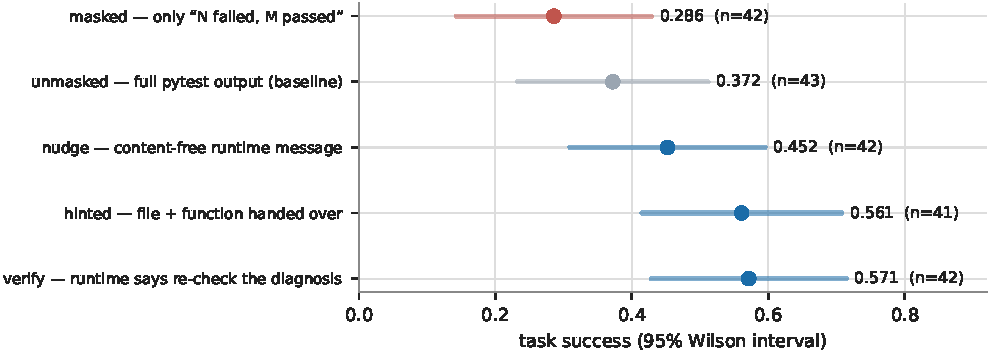
\includegraphics[width=\linewidth]{figures/fig7_live_conditions.pdf}
\caption{Only the comparisons involving \emph{masked} reach significance. Both runtime interventions
point the right way but neither is individually significant at this sample size.}
\label{fig:live_conditions}
\end{figure}

\noindent Two conclusions survive, and they are both narrower than the one we wanted. First, the
one solid causal result is about the \emph{benchmark}: hiding which tests failed costs 27.5 points
while the other conditions are statistically indistinguishable from each other. Second, the runtime
actions the router prescribes both point the right way --- a hint or a forced re-check is worth
roughly $+0.2$ over doing nothing, and the re-check costs no turn budget (11.1 turns against 12.2)
--- but \textbf{this experiment cannot attribute the gain to the instruction rather than to being
interrupted}, because a content-free message at the same moment moves success almost as far. A
clean separation needs a larger $n$ than this suite can supply, and we would rather report the
ambiguity than pick the attractive reading. Figure~\ref{fig:live_conditions} shows the five
conditions with Wilson intervals.

\paragraph{The router on live runs, and another negative.}
The frozen model was then applied unchanged to these episodes --- a different scaffold, a different
model, real packages --- and it does \textbf{not} transfer: AUC \textbf{0.426} at the 20\%
checkpoint ($n=125$) against 0.584 for the published output-overlap baseline. Re-fitting on the
training corpus with only the features that survive the transcript bridge, and dropping the
observation-scale family, recovers 0.602. This is the same conclusion the three external corpora
reached in \S4.4, from a completely different direction, and it is the reason the claim in this
paper is bounded to one scaffold's shards.

\noindent\emph{Note: the masked condition's first run produced 0/48 success and 0\% reaching the
gold file. That was a \textbf{harness fault, not a result}: every episode died before its first tool
call because the recorded Python interpreter had been deleted from a temp directory between runs.
No tokens were spent. It is recorded because the number has exactly the shape of a spectacular
finding and had to be checked against the transcripts to be disbelieved. The environment has been
rebuilt in-repo and the condition re-run; the numbers above are the corrected ones.}

\paragraph{Harness faults we had to fix, because they looked like results.}
(i) \textbf{65.2\% of turns were unparseable} in the first pilot --- our protocol was ad-hoc text,
but the model emits its own XML tool-call format regardless; native function-calling took this to
0--4\%. (ii) \textbf{The agent was writing its own tests into \code{tests/}}, which pytest collects,
so an agent-authored passing test could have scored a run as successful \emph{without the defect
being fixed}; the verifier is now restored to the packages' originals before grading, and in 72 of
84 valid episodes the agent had modified test files (1{,}076 files removed). (iii) the deleted
interpreter, above.

% =====================================================================================
\section{The demo}

\begin{quote}\small\ttfamily
python demo/route.py --fit \# train on shards 0--3, cache the model\\
python demo/route.py --summary \# router vs baselines on held-out shards\\
python demo/route.py --list \# held-out runs with their true modes\\
python demo/route.py --replay <run\_id> \# step through one run, turn by turn
\end{quote}

\noindent Offline, deterministic, no API key, and it reproduces the held-out numbers on demand.

% =====================================================================================
\section{Limitations}

\begin{itemize}[leftmargin=1.3em,itemsep=1pt]
\item \textbf{The cross-scaffold limit is severe, and we measured it rather than assuming it}
  (\S4.4). Every mechanical measurement rests on a structural footer SWE-agent prints into its
  observations (\code{[File: ... (N lines total)]}) in 95.8\% of edit steps. That footer is
  \textbf{absent from every other scaffold tested} --- OpenHands, the PI agent, mini-swe-agent-plus
  and a multi-framework corpus all show 0\% --- and the failure head trained on SWE-agent scores
  \textbf{0.319--0.495} on 88{,}000 runs from three other scaffolds. \textbf{Scaffold-independent
  generality is not claimed and this is the evidence against it.}
\item \textbf{The dead-end rate is scaffold-specific, not a property of coding agents}. Four other
  scaffolds, measured by the same mechanical rule: OpenHands \textbf{3.7\%}, the PI agent
  \textbf{11.8\%}, a multi-framework corpus \textbf{17.9\%}, mini-swe-agent-plus \textbf{23.6\%} ---
  a factor of six, and it moves in both directions away from SWE-agent. \textbf{19.1\% is
  SWE-agent's number and is not claimed for coding agents in general.}
\item \textbf{The 3.7\% figure rests on patch recovery from the transcript} for a scaffold with no
  printed patch; reported as a discrepancy to investigate.
\item \textbf{Step-level telemetry does not track what a person calls progress.} An independent
  blinded reader judged 12 windows (pre-registered, sealed key, one pass): agreement with the
  stored reader-produced judgements was \textbf{83.3\%} (Wilson [55.2, 95.3], $\kappa$ = +0.667)
  but with the mechanical progress measure only \textbf{50.0\%} ([25.4, 74.6], $\kappa$ = +0.100),
  with the disagreement concentrated on windows where the workspace moved without advancing the
  task. The labels used in \emph{this} paper do not depend on that measure --- they are defined
  against the dataset's gold patch --- but the pilot is why we do not claim that telemetry tracks
  progress, and it bounds what any behavioural monitor of this family can be expected to detect.
\item \textbf{The mode labels are coarse.} ``Ever touched a gold file'' is a proxy, not a judgement
  of fix quality; gold matching is basename-based and 4.10\% of edit steps carry no filename, which
  biases LOST upward.
\item \textbf{The live experiment is small} ($n = 41$--$43$ per condition, five conditions). The
  only comparisons that reach significance involve the masked condition (withholding the failure
  location costs $0.275$, $p = 0.015$). Both runtime interventions point the right way
  ($+0.189$ for the hint, $+0.199$ for the forced re-check) but neither is individually significant
  ($p = 0.125$, $p = 0.084$), and the content-free control is not distinguishable from the
  instruction it controls for ($p = 0.383$). The experiment is reported as \emph{suggestive of the
  interventions and conclusive only about the benchmark}.
\item \textbf{The inversion's mechanism is unexplained}: three candidates tested, all failed.
\item \textbf{Temperature-0 inference is not deterministic} ($\sim$9\% of per-instance outcomes flip
  across repeats), so within-instance comparisons are reported with runs-per-instance (mean 21.9).
\item \textbf{The corpus is 80{,}035 runs across three disjoint tables}, not one merged table. The
  single-table rebuild was attempted, failed, and the failure is recorded.
\end{itemize}

% =====================================================================================
\section{Reproducibility}

Six automated gates run on every change: invariant tests 11/11; cross-artifact consistency passes;
28/28 headline claims trace to their artifacts; 0 mismatches against the one-page summary; every
cited artifact exists; and 65/65 paper numbers trace to the artifact each one names. That last gate
was written during this work and \textbf{found five real errors in our own manuscript} --- values
quoted as pooled that were within-instance, figures mixed across two artifacts' row sets, and a
transfer table whose cells had been read off the wrong rows. All are fixed. Complete data package:
\code{research/EXPORT/}.

% =====================================================================================
\section{Use of AI tools}

A language model (\code{deepseek-v4.1-flash}) was used as a research assistant throughout ---
writing analysis code, running statistical tests, retrieving and verifying literature, and drafting
text. Every load-bearing citation was then verified by hand against the primary source, and two
reconnaissance claims were rejected as unverifiable. The model also served as the \emph{subject} of
the live experiment. It was not used to generate data; all measurements come from public corpora and
real test suites executed locally. \textbf{Eleven of its own claims were falsified and retracted},
documented pass by pass in the project's assistance log. Full disclosure, including the required
chat records, is in the separate acknowledgement and disclosure document.

% =====================================================================================
\newpage
\begin{thebibliography}{99}\small
\bibitem{agentstop} Pham et al. \emph{Terminating Local AI Agents Early to Save Energy in Consumer
Devices.} arXiv:2605.15206.
\bibitem{fap} \emph{Failure as a Process.} arXiv:2607.09510.
\bibitem{redundancy} \emph{RedundancyBench.} arXiv:2605.29893.
\bibitem{coherence} Mehta et al. \emph{Coherence Collapse: Diagnosing Why Code Agents Fail After
Reaching the Right Code.} arXiv:2603.24631.
\bibitem{confidentwrong} Mehta. \emph{Confident and Wrong: Silent Semantic Failures in Coding
Agents.} arXiv:2603.25764.
\bibitem{behaviour} \emph{Understanding Code Agent Behaviour: An Empirical Study of Success and
Failure Trajectories.} arXiv:2511.00197.
\bibitem{failforge} \emph{FailForge.} arXiv:2608.08570.
\bibitem{trim} \emph{TRIM: Reducing AI-Generated CodeSlop via Agent Trajectory Minimization.}
arXiv:2607.18161.
\bibitem{whowhen} Zhu et al. \emph{Which Agent Causes Task Failures and When?} arXiv:2505.00212.
\bibitem{noise} \emph{Temperature-0 nondeterminism on SWE-bench Verified.} arXiv:2607.09691.
\end{thebibliography}

% --- mandatory acknowledgement page (1-2 pages, 500-1500 characters) -----------------
\newpage
\section*{致谢与人工智能使用声明\\\large Acknowledgement and Disclosure of AI Use}
\addcontentsline{toc}{section}{致谢与人工智能使用声明 (Acknowledgement / AI disclosure)}

\subsection*{一、研究背景}

本项目研究编码智能体（coding agent）的失败方式，以及运行时系统能否在失败发生\emph{之前}判断智能体
究竟是「找不到代码」（LOST）还是「找到了代码但修改不正确」（WRONG-FIX）——因为这两种情况需要\emph{相反}
的干预措施。研究使用的数据全部来自公开的智能体运行轨迹数据集（SWE-agent / SWE-rebench、
Terminal-Bench 2.0，以及另外四个开源脚手架），以及八个开源 Python 软件包在本机运行的测试套件。
不涉及人类受试者，不使用任何非公开数据。

\subsection*{二、指导老师与参赛学生的关系}

[待填写] 四项缺一不可：
\begin{itemize}[leftmargin=1.3em,itemsep=1pt]
  \item 老师姓名与所在单位：\ [待填写]
  \item 学生与老师的结识渠道：\ [待填写]
  \item 指导有偿还是无偿（有偿须写明费用与来源）：\ [待填写]
  \item 老师参与与未参与的部分：\ [待填写]
\end{itemize}

\subsection*{三、分工说明}

本节写清\textbf{每位}作者的具体贡献。下述两项工作属于作者二（Xuhao Chen）而非外部协助，因此在此
列出，而非列入「来自他人的帮助」。

\begin{itemize}[leftmargin=1.3em,itemsep=2pt]
  \item \textbf{选题来源}：\ [待填写]
  \item \textbf{数据获取}：\ [待填写]
  \item \textbf{分析与计算}：\ [待填写]
  \item \textbf{实验设计与实施}：\ [待填写]
  \item \textbf{独立的盲评人机对照试验（作者二 Xuhao Chen）}：由作者二设计并实施——编写盲评窗口
        包与评分脚本（仅用标准库，含 Wilson 区间、$\kappa$、McNemar 检验）、预先注册判定规则、
        密封答案并在全部判定提交后才开封。结果为：人工判定与读者标注一致率 83.3\%（$\kappa$ =
        +0.667），与机械指标一致率仅 50.0\%（$\kappa$ = +0.100）。
  \item \textbf{数据重复问题的发现与修正（作者二 Xuhao Chen）}：由作者二发现 Terminal-Bench 2.0
        数据集中存在重复试验条目并给出去重规则；据此重建数据表，并重新计算受影响的全部统计量。
  \item \textbf{撰写论文}：\ [待填写]
  \item \textbf{遇到的困难及解决经过}：\ [待填写]
\end{itemize}

\subsection*{四、人工智能使用情况}

\textbf{工具与版本}：\texttt{deepseek-v4.1-flash}（大语言模型），通过 DeepSeek Harness（DSH）
自主编码助手接口调用。每一次模型调用的时间戳、token 数与费用均记录在
\texttt{research/results/rebuild/llm\_ledger.jsonl} 中；活体实验（241 次运行、5 种条件、48 个任务）
共花费 \textbf{2.26 美元}。

\textbf{使用阶段与用途}：（1）文献检索与核实（每条关键引文均由人工回原文献核对，其中两条前期结论
因无法查证而被剔除）；（2）编写轨迹解析与数据表构建代码；（3）编写并运行统计分析（任务不交叉的交叉
验证、自助法区间、Wilcoxon 检验、校准曲线、决策曲线）；（4）在活体实验中，模型本身是被测试的\emph{对象}；
（5）编写初稿文字，由参赛学生审阅并重写。

\textbf{时间与频率}：\textbf{2026 年 9 月 10 日至 9 月 13 日}，共四个工作时段，累计 34 次，逐次
记录于项目内的 AI 使用日志（\texttt{AI\_ASSISTANCE\_LOG.md}）。

\textbf{聊天记录}：按组委会要求另行提交。

\subsection*{五、来自他人的帮助}

[待填写] 本节只填\textbf{两位作者之外}的帮助；确无此类帮助，请写明「无」。（盲评试验中被判定的
12 个窗口，其判定人若在两位作者之外，请在此写明姓名。）

\subsection*{六、关于 AI 出错的自愿声明}

为如实说明研究的可信度，我们列出 AI 助手自身被推翻的\textbf{十一项}结论，包括：一个自指的定位指标
使结论方向相反；一项「零误报」声称属于循环论证；一项基线实际上等于运行长度；一次活体实验出现
「48 次全部失败」的惊人结果，实为解释器被删除的实验故障；论文中一张移植结果表引用了错误的数据行
（由自动审计脚本发现）；以及 Terminal-Bench 数据集的重复条目导致运行数与步数被高估（34{,}029 与
1{,}073{,}923 修正为 29{,}103 与 887{,}137，由合作者发现）。这说明本项目的规则是：\emph{只有当试图
推翻某结论的检验失败时，该结论才被保留}。全部十一项均逐次记录在
\texttt{research/AI\_ASSISTANCE\_LOG.md} 中。

\subsection*{七、声明}

我们声明：本文所述研究成果为参赛学生的原创工作；引用他人成果均已注明并在参考文献中列出；上述
人工智能使用情况完整、真实；我们已知悉并遵守本届竞赛的学术诚信规定。

\vspace{1.2em}
\noindent
\begin{tabular}{ll}
参赛学生签名： & \underline{\hspace{4.5cm}} \quad \underline{\hspace{4.5cm}} \\[10pt]
              & \hfill Ziheng Yu \hspace{2.2cm} Xuhao Chen \\[14pt]
指导老师签名： & \underline{\hspace{4.5cm}} \\[14pt]
日期：        & \underline{\hspace{4.5cm}} \\
\end{tabular}


\end{document}
